\documentclass[11pt]{article}
\usepackage[margin=1in]{geometry}
\usepackage{amsmath,amssymb,amsthm}
\usepackage{booktabs}
\usepackage{graphicx}
\usepackage{multicol}
\usepackage[hidelinks]{hyperref}
\usepackage{url}

\newtheorem{theorem}{Theorem}
\newtheorem{lemma}[theorem]{Lemma}
\theoremstyle{remark}
\newtheorem{remark}[theorem]{Remark}

\title{Smaller 5-chromatic unit-distance graphs\\ on two icosahedral spheres}
\author{Chandan Kumar Shukla\\ {\small Independent Researcher, India}\\ {\small \texttt{shukla.chandan12@gmail.com}}}
\date{}

\begin{document}
\maketitle

\begin{abstract}
Voronov, Neopryatnaya and Dergachev constructed 5-chromatic unit-distance graphs on the sphere
$S^2(r_1)$, $r_1=\cos\frac{\pi}{10}$, with $372$ vertices, and on $S^2(r_2)$, $r_2=\cos\frac{3\pi}{10}$,
with $972$ vertices, and noted that the first graph stays 5-chromatic after deleting any single vertex. By
SAT-based vertex minimization we find a 5-chromatic subgraph of the first graph with $231$ vertices and
$938$ edges, and one of the second with $961$ vertices and $4028$ edges. Both are vertex-critical and
contain no Moser spindle; the smaller one is the best found by our search, not a proved minimum. All
coordinates are given exactly in nested radicals and verified in exact arithmetic;
non-4-colourability is certified by DRAT proofs checked with \textsc{drat-trim}.
\end{abstract}

\section{Introduction}

The chromatic number $\chi(X)$ of a subset $X\subseteq\mathbb{R}^n$ is the least number of colours needed
to colour $X$ so that no two points at Euclidean distance $1$ receive the same colour. For the plane, de
Grey~\cite{deGrey} proved $\chi(\mathbb{R}^2)\ge5$; the smallest known 5-chromatic unit-distance graph in
the plane has $509$ vertices~\cite{Parts1} (see also~\cite{Heule1}).

For the sphere $S^2(r)\subset\mathbb{R}^3$ of radius $r>\tfrac12$, Simmons~\cite{Simmons} studied
colourings, and Voronov, Neopryatnaya and Dergachev~\cite{VND2022} constructed the first 5-chromatic unit-distance
graphs embedded in spheres, $G_{372}\subset S^2(r_1)$ and $G_{972}\subset S^2(r_2)$, where
$r_1=\cos\frac{\pi}{10}$ and $r_2=\cos\frac{3\pi}{10}$, proving $\chi(S^2(r_1))\ge5$ and
$\chi(S^2(r_2))\ge5$. They remark that $\chi(G_{372})=5$ is preserved after deleting any single vertex
and that they ``do not give here the subgraphs of $G_{372}$ that have the property of
minimality''~\cite[Sect.~4]{VND2022}. Cherkashin and Voronov~\cite{CV2022} ask, more generally, for the
minimal number of vertices of a subgraph $G$ of $S^2(r)$ with $\chi(G)=\chi(S^2(r))$.
We reduce both constructions.

\begin{theorem}\label{thm:main}
\begin{enumerate}
  \item[(a)] The graph $H_{231}\subset G_{372}$ defined in Section~\ref{sec:graphs} is a unit-distance
  graph in $S^2(r_1)$ with $231$ vertices and $938$ edges, and $\chi(H_{231})=5$.
  \item[(b)] The graph $H_{961}\subset G_{972}$ defined in Section~\ref{sec:graphs} is a unit-distance
  graph in $S^2(r_2)$ with $961$ vertices and $4028$ edges, and $\chi(H_{961})=5$.
\end{enumerate}
Both graphs are vertex-critical, i.e.\ deleting any vertex leaves a 4-colourable graph, and neither
contains the Moser spindle as a subgraph.
\end{theorem}

Thus $H_{231}$ has $38\%$ fewer vertices than $G_{372}$, while $G_{972}$ turns out to be nearly
vertex-critical (Remark~\ref{rem:972}). We do not know whether $231$ is the least order of a 5-chromatic
subgraph of $G_{372}$; it is the smallest our search found. Since $G_{372}$ and $G_{972}$ are defined exactly
in~\cite{VND2022}, our graphs are specified exactly by listing which of their vertices are kept or
removed (Section~\ref{sec:graphs}; all $231$ vertices of $H_{231}$ are listed in nested radicals in Appendix~S1 of the Supplementary Material).

\section{The parent graphs}\label{sec:parents}

Let $\Gamma$ be the full symmetry group of the regular icosahedron (order $120$, including reflections),
generated as in~\cite{VNDrepo} by
\[
\begin{pmatrix}-1&0&0\\0&-1&0\\0&0&1\end{pmatrix},\quad
\begin{pmatrix}0&0&1\\1&0&0\\0&1&0\end{pmatrix},\quad
\frac12\begin{pmatrix}1&-\tau&\tau^{-1}\\ \tau&\tau^{-1}&-1\\ \tau^{-1}&1&\tau\end{pmatrix},\quad
\begin{pmatrix}1&0&0\\0&-1&0\\0&0&1\end{pmatrix},
\qquad \tau=\tfrac{1+\sqrt5}{2}.
\]

\paragraph{$G_{372}$.} Its vertices are the $12$ vertices of the icosahedron with unit edge (the
$\Gamma$-orbit of $(\frac{\tau}{2},\frac12,0)$) together with the $\Gamma$-orbits of the three points
$v_1,v_2,v_3\in S^2(r_1)$ of Table~\ref{tab:poly372}, each orbit of size $120$; edges join vertices at
distance $1$. It has $372$ vertices and $1710$ edges~\cite{VND2022}.

\begin{table}[ht]
\centering\small
\begin{tabular}{ccl}
\toprule
 & value & minimal polynomial of twice the coordinate \\
\midrule
$x_1$ & $\phantom{-}0.71584\ldots$ & $x^4-2x^3+2x^2-x-1$ \\
$y_1$ & $\phantom{-}0.34924\ldots$ & $x^4+x^3-2x^2+2x-1$ \\
$z_1$ & $\phantom{-}0.51972\ldots$ & $x^8-5x^6+2x^4+20x^2-19$ \\
$x_2,\ x_3$ & $-0.07961\ldots,\ -0.17646\ldots$ & $x^8-x^7-4x^6+6x^5+28x^4-7x^3+9x^2+8x+1$ \\
$y_2,\ y_3$ & $-0.08345\ldots,\ \phantom{-}0.79929\ldots$ & $x^8-2x^7+x^6-5x^5+9x^4-4x^3+5x^2-5x-1$ \\
$z_2$ & $\phantom{-}0.94404\ldots$ & $x^8-3x^7+10x^5+4x^4-24x^3-13x^2+7x-1$ \\
$z_3$ & $\phantom{-}0.48426\ldots$ & $x^8+3x^7-10x^5+4x^4+24x^3-13x^2-7x-1$ \\
\bottomrule
\end{tabular}
\caption{Orbit representatives $v_i=(x_i,y_i,z_i)$ of $G_{372}$, from~\cite{VND2022}.}
\label{tab:poly372}
\end{table}

\paragraph{$G_{972}$.} Its vertices are the $12$ vertices of the great icosahedron with unit edge (the
$\Gamma'$-orbit of $\tau^{-1}(\frac12,\frac{\tau}{2},0)$, where $\Gamma'$ is $\Gamma$ conjugated by the
coordinate swap $y\leftrightarrow z$, as in~\cite{VNDrepo}) together with the $\Gamma'$-orbits of eight
points $w_1,\dots,w_8\in S^2(r_2)$, each of size $120$. The coordinates of $w_i$ are given
in~\cite{VNDrepo} as roots of explicit polynomials of degree $8$ (reproduced in the repository, \texttt{construction/build\_G972.py});
for instance the second coordinate of $w_8$ is
$\frac14\bigl(1-\sqrt{6-3\sqrt5+2\sqrt{(17\sqrt5-37)/2}}\bigr)$. The graph has $972$ vertices and $4110$
edges.

\begin{lemma}\label{rem:field}
For each sphere, all coordinates of all vertices of the parent graph lie in a number field $K$ of degree
$8$ whose Galois closure has group $D_8$ (of order $16$). Consequently $K$ is a tower of quadratic
extensions $\mathbb{Q}\subset\mathbb{Q}(\sqrt5)\subset\mathbb{Q}(\sqrt5,b)\subset\mathbb{Q}(\sqrt5,b,g)=K$
with $b=\sqrt\beta$, $g=\sqrt\gamma$, where
\begin{align*}
S^2(r_1):\quad & \beta=\tfrac72+\tfrac52\sqrt5,\qquad
\gamma=\tfrac{15}{4}-\tfrac74\sqrt5+\bigl(\tfrac34-\tfrac14\sqrt5\bigr)b,\\
S^2(r_2):\quad & \beta=\tfrac{23}{2}+\tfrac{11}{2}\sqrt5,\qquad
\gamma=\tfrac54-\tfrac34\sqrt5+\bigl(-\tfrac14+\tfrac14\sqrt5\bigr)b,
\end{align*}
all square roots being positive. Every coordinate of every vertex is a $\mathbb{Q}$-linear combination of
$1,\sqrt5,b,\sqrt5 b,g,\sqrt5 g,bg,\sqrt5 bg$, i.e.\ an explicit nested radical with rational
coefficients. For example, vertex~13 of $H_{231}$ (Appendix~S1 of the Supplementary Material) is
\[
\Bigl(\tfrac14+\tfrac{\sqrt5-1}{8}\,b,\ \ -\tfrac{1+\sqrt5}{8}+\tfrac14\,b,\ \ \tfrac{1+\sqrt5}{4}\,g\Bigr)
\qquad\text{on }S^2(r_1).
\]
\end{lemma}
The field and the tower were computed with PARI/GP~\cite{PARI}; the exact coordinates of all vertices of
$H_{231}$ and $H_{961}$ in this form, written with integers, fractions and square roots only, are in the
repository (Mathematica and Python syntax).

\section{The graphs $H_{231}$ and $H_{961}$}\label{sec:graphs}

The exact coordinates of every vertex are given as nested radicals (Lemma~\ref{rem:field}) in the
repository. For readability, the tables below list coordinates rounded to four decimals; since
the vertices of $G_{372}$ are pairwise at distance at least $0.049$, and those of $G_{972}$ at least
$0.009$, these rounded triples identify the exact vertices unambiguously. Exact radical forms of the orbit representatives are given in Appendix~\ref{app:reps}.

\paragraph{$H_{231}$} is the subgraph of $G_{372}$ induced by the $231$ vertices listed, with exact coordinates in nested radicals and a
5-colouring, in Appendix~S1 of the Supplementary Material: all $12$ icosahedron vertices, $99$ vertices of the orbit of $v_1$, and $60$
vertices of each of the orbits of $v_2$ and $v_3$. Its symmetry group within $\Gamma$ is trivial.

\paragraph{$H_{961}$} is obtained from $G_{972}$ by deleting the $11$ vertices of Table~\ref{tab:removed}.

\begin{table}[ht]
\centering\small
\begin{tabular}{rlrrr}
\toprule
 & orbit & $x$ & $y$ & $z$\\
\midrule
1 & $w_3$-orbit & $-0.1495$ & $-0.4014$ & $\phantom{-}0.4025$ \\
2 & $w_4$-orbit & $\phantom{-}0.5257$ & $\phantom{-}0.1359$ & $-0.2250$ \\
3 & $w_4$-orbit & $-0.1650$ & $\phantom{-}0.5628$ & $-0.0388$ \\
4 & $w_4$-orbit & $\phantom{-}0.1228$ & $\phantom{-}0.3849$ & $\phantom{-}0.4269$ \\
5 & $w_4$-orbit & $-0.1599$ & $\phantom{-}0.2878$ & $\phantom{-}0.4869$ \\
6 & $w_4$-orbit & $\phantom{-}0.2250$ & $-0.5257$ & $-0.1359$ \\
7 & $w_4$-orbit & $\phantom{-}0.4869$ & $-0.1599$ & $\phantom{-}0.2878$ \\
8 & $w_4$-orbit & $\phantom{-}0.0600$ & $\phantom{-}0.4237$ & $-0.4029$ \\
9 & $w_4$-orbit & $-0.3849$ & $-0.4269$ & $-0.1228$ \\
10 & $w_4$-orbit & $\phantom{-}0.5628$ & $\phantom{-}0.0388$ & $\phantom{-}0.1650$ \\
11 & $w_4$-orbit & $-0.4237$ & $-0.4029$ & $-0.0600$ \\
\bottomrule
\end{tabular}
\caption{The $11$ vertices of $G_{972}$ deleted to obtain $H_{961}$ (four-decimal labels).}
\label{tab:removed}
\end{table}

Table~\ref{tab:summary} summarizes both graphs and Figure~\ref{fig:h231} shows $H_{231}$.

\begin{table}[ht]
\centering\small
\begin{tabular}{lcccccc}
\toprule
graph & sphere & $|V|$ & $|E|$ & degrees & composition by orbit & vertex-critical \\
\midrule
$G_{372}$~\cite{VND2022} & $S^2(r_1)$ & 372 & 1710 & & $12+120+120+120$ & no \\
$H_{231}$ & $S^2(r_1)$ & 231 & 938 & 4--25 (avg.\ 8.12) & $12+99+60+60$ & yes \\
\midrule
$G_{972}$~\cite{VND2022} & $S^2(r_2)$ & 972 & 4110 & & $12+8\times120$ & no \\
$H_{961}$ & $S^2(r_2)$ & 961 & 4028 & 5--65 (avg.\ 8.38) & $12+8\times120-11$ & yes \\
\bottomrule
\end{tabular}
\caption{The parent graphs and the reduced graphs.}
\label{tab:summary}
\end{table}

\begin{figure}[ht]
\centering
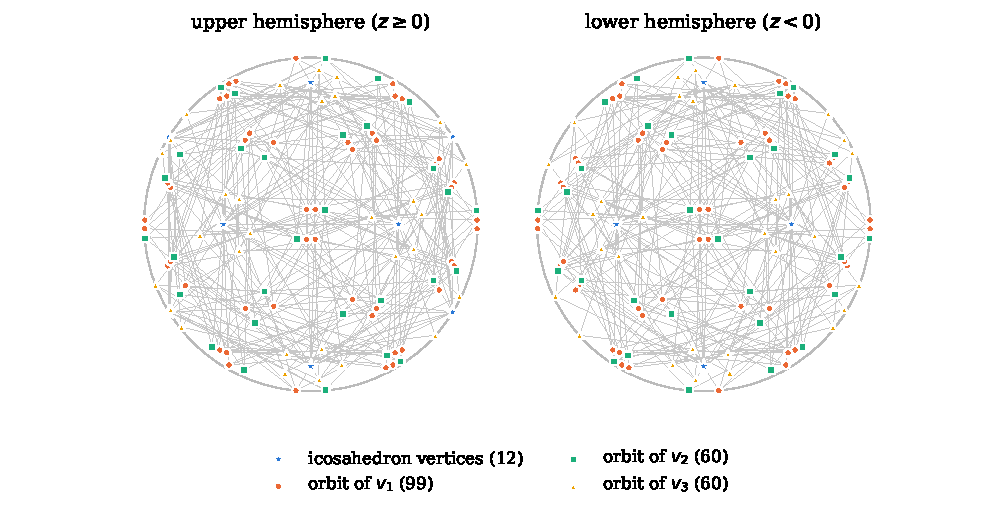
\includegraphics[width=\textwidth]{fig_h231.pdf}
\caption{Orthogonal projections of $H_{231}$ onto the $xy$-plane: vertices with $z\ge0$ (left) and
$z<0$ (right, viewed from below). Marker shape and colour indicate the orbit of $G_{372}$ a vertex
belongs to; edges between vertices of the same hemisphere are drawn in grey. The bounding circle has
radius $r_1$.}
\label{fig:h231}
\end{figure}

\section{Proof of Theorem~\ref{thm:main}}\label{sec:proof}

The proof has four parts; parts (ii)--(iv) are finite computations, each accompanied by a certificate
that can be checked independently of the software that produced it.

\paragraph{(i) Embedding and edges.} By Lemma~\ref{rem:field} all vertices have coordinates in a field
$K$ of degree $8$. In PARI/GP~\cite{PARI} we represent $K$ as $\mathbb{Q}[y]/(F(y))$, compute each
coordinate of every orbit representative as an element of $K$ (the roots of the minimal polynomials in
$K$, choosing the real embedding of $K$ that matches the numerical values), generate the $120$ matrices
of $\Gamma$ (resp.\ $\Gamma'$) exactly, and form all vertices. For every vertex $p$ of $H_{231}$ and
$H_{961}$ we check $p\cdot p=r^2$ exactly, with $r_1^2=\frac{5+\sqrt5}{8}$ and
$r_2^2=\frac{5-\sqrt5}{8}$, and for every edge $pq$ we check $|p-q|^2=1$ exactly ($938$ and $4028$
identities in $K$; all hold). Conversely, no unit distance is missing: with the coordinates to $30$ significant digits
(files \texttt{H231\_vertices.txt}, \texttt{H961\_vertices.txt}), every non-adjacent pair satisfies $\bigl||p-q|-1\bigr|\ge 2.2\cdot10^{-3}$ in
$H_{231}$ and $\ge4.1\cdot10^{-4}$ in $H_{961}$, far above the numerical error. Hence both graphs are
unit-distance graphs on the stated spheres with the stated numbers of edges.

This was double-checked independently of PARI/GP: a short program implements exact arithmetic in the
basis $1,\sqrt5,b,\sqrt5b,g,\sqrt5g,bg,\sqrt5bg$ with rational coefficients (using only the relations
$\sqrt5^2=5$, $b^2=\beta$, $g^2=\gamma$), reads the nested-radical coordinates from the files
\texttt{H231\_exact\_coordinates.m} and \texttt{H961\_exact\_coordinates.m}, and confirms $p\cdot p=r^2$ for all vertices and $|p-q|^2=1$ for all $938$ and $4028$ edges; as a
negative control, perturbing a single coordinate by $10^{-3}$ is detected (the vertex leaves the sphere
and all its edges fail). The edges also form a subset of the edges of $G_{372}$ and $G_{972}$, whose unit
distances were verified symbolically in~\cite{VND2022,VNDrepo}.

\paragraph{(ii) No proper 4-colouring.} We encode the existence of a proper 4-colouring as a CNF formula
with variables $x_{v,c}$, clauses $\bigvee_{c}x_{v,c}$ and $\neg x_{v,c}\vee\neg x_{v,c'}$ ($c\ne c'$)
for every vertex $v$, clauses $\neg x_{u,c}\vee\neg x_{v,c}$ for every edge $uv$ and colour $c$, and two
unit clauses fixing the colours of the endpoints of one edge (which loses no generality). The SAT solver
\textsc{Kissat}~\cite{Kissat} reports both formulas unsatisfiable and emits proofs in the DRAT format;
the independent checker \textsc{drat-trim}~\cite{WetzlerHeuleHunt2014} validates both proofs
(\texttt{s VERIFIED}; files \texttt{H231\_4col.cnf}, \texttt{H231\_4col.drat.xz} and likewise for $H_{961}$). As further independent confirmation, the solvers CaDiCaL, Glucose and MiniSat (via
PySAT~\cite{PySAT}) and a second encoding with two Boolean variables per vertex give the same answer
(\texttt{verification/crosscheck\_solvers.py}), and
for $H_{231}$ a plain backtracking search (DSATUR vertex order, colour-symmetry breaking, about
$7\cdot10^{6}$ nodes, no SAT solver) finds no proper 4-colouring. Hence $\chi\ge5$.

\paragraph{(iii) A proper 5-colouring.} A 5-colouring of $H_{231}$ is listed in Appendix~S1 of the Supplementary Material
(colour classes of sizes $55,51,49,46,30$); both colourings are in the files \texttt{H231\_5colouring.txt} and
\texttt{H961\_5colouring.txt} and were checked edge by edge. Hence $\chi=5$.

\paragraph{(iv) Criticality and spindles.} For each vertex $v$ the files
\texttt{H231\_criticality\_certificates.txt} and \texttt{H961\_criticality\_certificates.txt} contain a
proper 4-colouring of the graph with $v$ deleted ($231$ and $961$ certificates); each was checked edge by
edge. Hence both graphs are vertex-critical. An exhaustive search over all pairs of rhombi (pairs of triangles sharing an edge)
with a common apex whose tips are adjacent finds no Moser spindle in either graph. \hfill$\square$

\section{How the graphs were found}\label{sec:method}

\paragraph{Encoding with selectors.} To test many vertex subsets $U\subseteq V$ we add a selector literal
$s_v$ to every at-least-one-colour clause, $\neg s_v\vee\bigvee_c x_{v,c}$, and solve under the
assumptions $\{s_v:v\in U\}$, with the colours of one triangle of $U$ fixed. An unsatisfiable answer comes
with a \emph{core}: a subset of the assumptions that is already unsatisfiable, i.e.\ a non-4-colourable
subset of $U$.

\paragraph{Algorithm 1 (random-order vertex deletion).}
\begin{enumerate}
\item Set $U\leftarrow V$ and $C\leftarrow\emptyset$ (vertices known to be essential).
\item Repeatedly remove vertices of degree $<4$ in $G[U]$ (they never affect 4-colourability).
\item Pick a random $v\in U\setminus C$. If $G[U\setminus\{v\}]$ is not 4-colourable, replace $U$ by the
returned core (and go to step 2); otherwise add $v$ to $C$.
\item Stop when $C=U$.
\end{enumerate}
Each test was run with a conflict limit and an inconclusive test was treated as ``4-colourable'', so the
output is vertex-critical only up to these limits; criticality of the final graphs $H_{231}$ and $H_{961}$
was verified separately (Section~\ref{sec:proof}).
For $G_{372}$ each test takes well under a second. Sixteen runs with different random orders gave
non-4-colourable subgraphs with between $235$ and $337$ vertices (Figure~\ref{fig:runs}).

\paragraph{Algorithm 2 (local search).} Starting from a vertex-critical $U$: add to $U$ between $5$ and $40$
random vertices of $V\setminus U$ having at least $2$ to $4$ neighbours in $U$, optionally delete a few
random vertices of $U$, run Algorithm~1 on the resulting set, and accept the result if it is not larger
than $U$. Starting from the $235$-vertex subgraph this produced the $231$-vertex graph $H_{231}$.

\paragraph{Triage for $G_{972}$.} For $G_{972}$ each test takes several seconds, so we first tested every
vertex $v$ of a 5-chromatic subgraph $U$ with $|U|=968$ separately. If $G[U\setminus\{v\}]$ is
4-colourable, then $v$ lies in every non-4-colourable subgraph of $G[U]$ and need never be tested again.
Only $34$ of the $968$ vertices were individually removable ($931$ were shown to be essential; the three
vertices of the triangle whose colours were fixed were not tested); deleting the $34$ greedily gave $963$
vertices, and Algorithm~2 gave $961$.

\begin{remark}\label{rem:972}
Unlike $G_{372}$, the graph $G_{972}$ is close to vertex-critical: at least $931$ of the $968$ vertices of
the first subgraph examined are essential.
\end{remark}

\begin{figure}[ht]
\centering
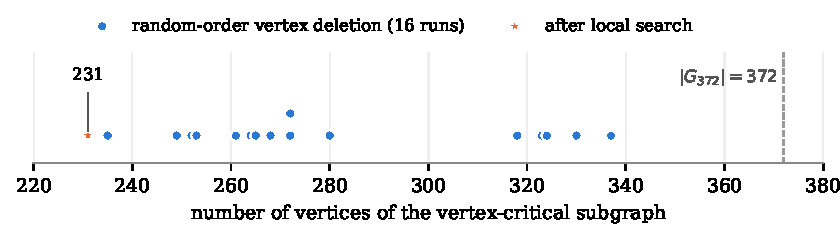
\includegraphics[width=0.85\textwidth]{fig_runs.pdf}
\caption{Sizes of the non-4-colourable subgraphs of $G_{372}$ found by $16$ runs of Algorithm~1 with
different random orders, and the result of Algorithm~2.}
\label{fig:runs}
\end{figure}

\section{Data availability}

All data, proofs and code are in the repository accompanying this paper (\url{https://github.com/chandanshukla1989/5chromatic-spheres}): for both graphs
the vertex lists (parent-graph indices and $30$-digit coordinates), exact coordinates in nested radicals
(Mathematica and Python syntax), edge lists, 5-colourings, criticality certificates, CNF formulas with
compressed DRAT proofs and \textsc{drat-trim} logs, the scripts that rebuild $G_{372}$ and $G_{972}$, and
the verification programs. A single script (\texttt{verify\_all.sh}) re-runs every check of
Section~\ref{sec:proof}. The Supplementary Material describes the files and procedures and lists all
coordinates in radicals.

\section{Concluding remarks}

The graph $H_{231}$ is a local optimum of our search; determining the smallest 5-chromatic subgraph of
$G_{372}$, or the smallest 5-chromatic unit-distance graph in $S^2(r_1)$, remains open. An exact
implicit-hitting-set computation of the former did not finish within the time we allotted. The other
constructions of~\cite{VND2022} may also contain much smaller 5-chromatic subgraphs.

\section*{Use of AI tools}
The author initiated and led this work, set its verification standards (exact algebraic coordinates and
certificate-based proofs) and takes full responsibility for all claims. AI tools were used for
computational exploration, for implementing the search and verification scripts, and for drafting the
text. Every claim rests on certificates or exact computations that can be re-checked independently
(Section~\ref{sec:proof}).

\bibliographystyle{plain}
\bibliography{refs}

\appendix
\section{Exact orbit representatives}\label{app:reps}

With $b=\sqrt\beta$ and $g=\sqrt\gamma$ as in Lemma~\ref{rem:field} (separately for each sphere, all
square roots positive), the orbit representatives $v_1,v_2,v_3$ of $G_{372}$ and $w_1,\dots,w_8$ of $G_{972}$ are as follows.
Every other vertex is the image of one of them under the symmetry group (or a vertex of the (great)
icosahedron), so these points determine all vertices exactly. The complete list of the $231$ vertices of
$H_{231}$ in nested radicals is in Appendix~S1 of the Supplementary Material; the $961$ vertices of $H_{961}$ are in
\texttt{H961\_exact\_coordinates.m}.

{\small
\paragraph{$v_{1}$} (on $S^2(r_1)$)
\begin{align*}
x&=\tfrac{1}{4}-\tfrac{1}{8}b+\tfrac{1}{8}\sqrt5\,b\\
y&=-\tfrac{1}{8}-\tfrac{1}{8}\sqrt5+\tfrac{1}{4}b\\
z&=\tfrac{1}{4}g+\tfrac{1}{4}\sqrt5\,g
\end{align*}

\paragraph{$v_{2}$} (on $S^2(r_1)$)
\begin{align*}
x&=\tfrac{1}{16}+\tfrac{3}{16}\sqrt5-\tfrac{1}{16}b-\tfrac{1}{16}\sqrt5\,b+\tfrac{5}{16}g+\tfrac{1}{16}\sqrt5\,g-\tfrac{1}{8}bg\\
y&=\tfrac{1}{8}-\tfrac{1}{16}b+\tfrac{1}{16}\sqrt5\,b+\tfrac{1}{16}g-\tfrac{1}{16}\sqrt5\,g-\tfrac{1}{16}bg-\tfrac{1}{16}\sqrt5\,bg\\
z&=\tfrac{3}{16}+\tfrac{3}{16}\sqrt5-\tfrac{1}{8}b+\tfrac{1}{8}g+\tfrac{3}{16}bg+\tfrac{1}{16}\sqrt5\,bg
\end{align*}

\paragraph{$v_{3}$} (on $S^2(r_1)$)
\begin{align*}
x&=\tfrac{1}{16}+\tfrac{3}{16}\sqrt5-\tfrac{1}{16}b-\tfrac{1}{16}\sqrt5\,b-\tfrac{5}{16}g-\tfrac{1}{16}\sqrt5\,g+\tfrac{1}{8}bg\\
y&=\tfrac{1}{8}-\tfrac{1}{16}b+\tfrac{1}{16}\sqrt5\,b-\tfrac{1}{16}g+\tfrac{1}{16}\sqrt5\,g+\tfrac{1}{16}bg+\tfrac{1}{16}\sqrt5\,bg\\
z&=-\tfrac{3}{16}-\tfrac{3}{16}\sqrt5+\tfrac{1}{8}b+\tfrac{1}{8}g+\tfrac{3}{16}bg+\tfrac{1}{16}\sqrt5\,bg
\end{align*}

\paragraph{$w_{1}$} (on $S^2(r_2)$)
\begin{align*}
x&=-\tfrac{5}{8}+\tfrac{1}{8}\sqrt5+\tfrac{3}{8}b-\tfrac{1}{8}\sqrt5\,b-\tfrac{3}{16}g+\tfrac{1}{16}\sqrt5\,g-\tfrac{1}{16}bg+\tfrac{1}{16}\sqrt5\,bg\\
y&=-\tfrac{1}{8}-\tfrac{1}{8}\sqrt5-\tfrac{1}{2}b+\tfrac{1}{4}\sqrt5\,b-\tfrac{1}{4}g+\tfrac{1}{8}\sqrt5\,g-\tfrac{3}{16}bg+\tfrac{1}{16}\sqrt5\,bg\\
z&=-\tfrac{5}{8}+\tfrac{1}{8}\sqrt5+\tfrac{3}{16}g+\tfrac{1}{16}\sqrt5\,g+\tfrac{1}{4}bg-\tfrac{1}{8}\sqrt5\,bg
\end{align*}

\paragraph{$w_{2}$} (on $S^2(r_2)$)
\begin{align*}
x&=-\tfrac{5}{8}+\tfrac{1}{8}\sqrt5+\tfrac{3}{8}b-\tfrac{1}{8}\sqrt5\,b+\tfrac{3}{16}g-\tfrac{1}{16}\sqrt5\,g+\tfrac{1}{16}bg-\tfrac{1}{16}\sqrt5\,bg\\
y&=-\tfrac{1}{8}-\tfrac{1}{8}\sqrt5-\tfrac{1}{2}b+\tfrac{1}{4}\sqrt5\,b+\tfrac{1}{4}g-\tfrac{1}{8}\sqrt5\,g+\tfrac{3}{16}bg-\tfrac{1}{16}\sqrt5\,bg\\
z&=\tfrac{5}{8}-\tfrac{1}{8}\sqrt5+\tfrac{3}{16}g+\tfrac{1}{16}\sqrt5\,g+\tfrac{1}{4}bg-\tfrac{1}{8}\sqrt5\,bg
\end{align*}

\paragraph{$w_{3}$} (on $S^2(r_2)$)
\begin{align*}
x&=-\tfrac{159}{656}-\tfrac{69}{656}\sqrt5-\tfrac{23}{328}b+\tfrac{7}{164}\sqrt5\,b+\tfrac{3}{164}g-\tfrac{9}{328}\sqrt5\,g+\tfrac{29}{656}bg-\tfrac{23}{656}\sqrt5\,bg\\
y&=-\tfrac{257}{656}+\tfrac{119}{656}\sqrt5+\tfrac{93}{656}b-\tfrac{37}{656}\sqrt5\,b-\tfrac{51}{656}g+\tfrac{15}{656}\sqrt5\,g-\tfrac{9}{82}bg+\tfrac{13}{328}\sqrt5\,bg\\
z&=-\tfrac{87}{328}+\tfrac{7}{82}\sqrt5-\tfrac{113}{656}b+\tfrac{67}{656}\sqrt5\,b+\tfrac{17}{656}g-\tfrac{87}{656}\sqrt5\,g-\tfrac{17}{656}bg+\tfrac{5}{656}\sqrt5\,bg
\end{align*}

\paragraph{$w_{4}$} (on $S^2(r_2)$)
\begin{align*}
x&=-\tfrac{159}{656}-\tfrac{69}{656}\sqrt5-\tfrac{23}{328}b+\tfrac{7}{164}\sqrt5\,b-\tfrac{3}{164}g+\tfrac{9}{328}\sqrt5\,g-\tfrac{29}{656}bg+\tfrac{23}{656}\sqrt5\,bg\\
y&=\tfrac{257}{656}-\tfrac{119}{656}\sqrt5-\tfrac{93}{656}b+\tfrac{37}{656}\sqrt5\,b-\tfrac{51}{656}g+\tfrac{15}{656}\sqrt5\,g-\tfrac{9}{82}bg+\tfrac{13}{328}\sqrt5\,bg\\
z&=\tfrac{87}{328}-\tfrac{7}{82}\sqrt5+\tfrac{113}{656}b-\tfrac{67}{656}\sqrt5\,b+\tfrac{17}{656}g-\tfrac{87}{656}\sqrt5\,g-\tfrac{17}{656}bg+\tfrac{5}{656}\sqrt5\,bg
\end{align*}

\paragraph{$w_{5}$} (on $S^2(r_2)$)
\begin{align*}
x&=-\tfrac{169}{656}+\tfrac{69}{656}\sqrt5+\tfrac{23}{328}b-\tfrac{7}{164}\sqrt5\,b-\tfrac{3}{164}g+\tfrac{9}{328}\sqrt5\,g-\tfrac{29}{656}bg+\tfrac{23}{656}\sqrt5\,bg\\
y&=\tfrac{93}{656}+\tfrac{45}{656}\sqrt5-\tfrac{93}{656}b+\tfrac{37}{656}\sqrt5\,b+\tfrac{51}{656}g-\tfrac{15}{656}\sqrt5\,g+\tfrac{9}{82}bg-\tfrac{13}{328}\sqrt5\,bg\\
z&=-\tfrac{9}{82}+\tfrac{13}{328}\sqrt5+\tfrac{31}{656}b+\tfrac{15}{656}\sqrt5\,b+\tfrac{147}{656}g-\tfrac{77}{656}\sqrt5\,g+\tfrac{17}{656}bg-\tfrac{5}{656}\sqrt5\,bg
\end{align*}

\paragraph{$w_{6}$} (on $S^2(r_2)$)
\begin{align*}
x&=-\tfrac{169}{656}+\tfrac{69}{656}\sqrt5+\tfrac{23}{328}b-\tfrac{7}{164}\sqrt5\,b+\tfrac{3}{164}g-\tfrac{9}{328}\sqrt5\,g+\tfrac{29}{656}bg-\tfrac{23}{656}\sqrt5\,bg\\
y&=\tfrac{93}{656}+\tfrac{45}{656}\sqrt5-\tfrac{93}{656}b+\tfrac{37}{656}\sqrt5\,b-\tfrac{51}{656}g+\tfrac{15}{656}\sqrt5\,g-\tfrac{9}{82}bg+\tfrac{13}{328}\sqrt5\,bg\\
z&=\tfrac{9}{82}-\tfrac{13}{328}\sqrt5-\tfrac{31}{656}b-\tfrac{15}{656}\sqrt5\,b+\tfrac{147}{656}g-\tfrac{77}{656}\sqrt5\,g+\tfrac{17}{656}bg-\tfrac{5}{656}\sqrt5\,bg
\end{align*}

\paragraph{$w_{7}$} (on $S^2(r_2)$)
\begin{align*}
x&=-\tfrac{3}{8}+\tfrac{3}{16}b-\tfrac{1}{16}\sqrt5\,b-\tfrac{3}{16}g+\tfrac{1}{16}\sqrt5\,g+\tfrac{1}{16}bg-\tfrac{1}{16}\sqrt5\,bg\\
y&=\tfrac{1}{16}-\tfrac{1}{16}\sqrt5+\tfrac{1}{4}b-\tfrac{1}{8}\sqrt5\,b-\tfrac{1}{4}g+\tfrac{1}{8}\sqrt5\,g+\tfrac{3}{16}bg-\tfrac{1}{16}\sqrt5\,bg\\
z&=-\tfrac{7}{16}+\tfrac{1}{16}\sqrt5-\tfrac{1}{16}b+\tfrac{1}{16}\sqrt5\,b-\tfrac{5}{16}g+\tfrac{1}{16}\sqrt5\,g-\tfrac{1}{4}bg+\tfrac{1}{8}\sqrt5\,bg
\end{align*}

\paragraph{$w_{8}$} (on $S^2(r_2)$)
\begin{align*}
x&=-\tfrac{3}{8}+\tfrac{1}{8}\sqrt5+\tfrac{3}{16}g-\tfrac{1}{16}\sqrt5\,g+\tfrac{1}{16}bg-\tfrac{1}{16}\sqrt5\,bg\\
y&=\tfrac{1}{4}-\tfrac{1}{4}g+\tfrac{1}{8}\sqrt5\,g-\tfrac{3}{16}bg+\tfrac{1}{16}\sqrt5\,bg\\
z&=-\tfrac{1}{8}-\tfrac{1}{8}\sqrt5+\tfrac{3}{8}b-\tfrac{1}{8}\sqrt5\,b+\tfrac{5}{16}g-\tfrac{1}{16}\sqrt5\,g-\tfrac{1}{4}bg+\tfrac{1}{8}\sqrt5\,bg
\end{align*}
}

\end{document}
